\section{Multi-tenancy}
\label{sec:multitenancy}   

One of the main decision variables for utilizing a Cloud computing environment are capital expenditures. The main goal of a Cloud consumer is to minimize its business costs when migrating to the Cloud. According to Chong, a \ac{SaaS} solution benefits a Cloud customer with the following advantages \cite{ChongB2006}:

	\begin{itemize}
		\item The Cloud consumer does not directly purchase a software license, but a subscription to the software offered as a service by the Cloud infrastructure. 
		\item More than half of the IT investments of a company are made in infrastructure and its maintenance. In a \ac{SaaS} solution this responsibilities are mainly externalized to the Cloud provider.   
		\item A Cloud computing environment is based on the utilization of its resources simultaneously by a large number of Cloud consumers. For example, a Cloud provider that offers a centrally-hosted software service to a large number of customers can serve all of them in a consolidated environment and lower the customer software subscription costs while maintaining or lowering the provider's infrastructure, administration and maintenance costs. 
		\item The cost leverage in the software utilization allows the Cloud providers to focus not only on big enterprises capable of large IT budgets, but also on the small business that need access to IT solutions. 
	\end{itemize} 

Multi-tenancy in a \ac{SaaS} environment allows the Cloud providers to lower the cost per customer by optimizing the resources usage in the Cloud infrastructure. The software serves multiple tenants concurrently, who share the same code base and data storage systems. Chong and Carraro \cite{ChongB2006} define a well designed \ac{SaaS} application as scalable, multi-tenant-efficient and configurable. With this design patterns, the \ac{SaaS} model enables the provider to \term{catch the long tail}. Business softwares are becoming more complex and tend to demand an individual customer support and an increase of the computing and storage resources in the infrastructure. This fact leads to an increase in the infrastructure investment and maintenance costs. However, if the previous requirements are eliminated and the provider's infrastructure is scaled to combine and centralize customers' hardware and services requirements, the price reduction limit can be decreased and, in effect, allow a wide range of consumers to be able to access this services.

The reasons discussed above are also applicable in the \ac{DBaaS} and \ac{STaaS} models. Storage and retrieval of data involve high maintenance and management costs. The data management cost is estimated to be between 5 to 10 times higher than the data gain cost \cite{multishares2011}. Furthermore, storing data on-premise does not only require storing and retrieving data, but also requires dealing with disaster recovery, \ac{DBMS}, capacity planning, etc. Most of the organizations prefer to lead their investments to their local business applications rather than becoming a data management company \cite{multishares2011}. Cloud storage providers offer a pay-per-use storage model, e.g. based on storage capacity or based on number of connections to the storage system, and ensure that the stored data will persist over time and its access through the network. However, security and confidentiality are the main constraints when moving private data to a shared public infrastructure. 

\begin{figure}[htb]
	\centering
		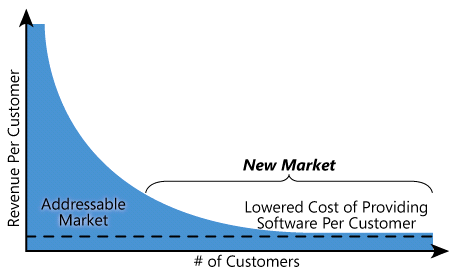
\includegraphics[clip, scale=0.5]{./gfx/longtail.png}
	\caption[Multi-tenancy and Long Tail]{New market opened by lower cost of SaaS \cite{ChongB2006}}
	\label{fig:longtail}
\end{figure}

In the Figure \ref{fig:longtail} the economics of scaling up to a high number of customers while reducing the software price is analyzed. Cloud providers have reached a new market formed by small or medium businesses without enough budget for building an on-premise IT infrastructure.

Multi-tenancy refers to the sharing of the whole technological stack (hardware, operating system, middleware, and application instances) at the same time by different tenants and their corresponding users \cite{EnablingMT}. Andrikopoulos et al. identify two fundamental aspects in multi-tenant awareness: communication, and administration and management \cite{andrikopoulos2013}. The former involves isolated message exchanges between tenants and the latter allows tenants individual configuration and management of their communication endpoints. Utilizing an \ac{ESB} as the central piece of communication middleware between applications in a \ac{PaaS} environment forces it to ensure multi-tenancy at both communication, and administration and management, as mentioned before. The multi-tenancy support modifications made in the open-source ServiceMix 4.3 are the results of \cite{Essl2011}, \cite{Muhler2012}, and \cite{gomez2012}. In this diploma thesis we reuse and extend those results in oder to provide multi-tenant transparent Cloud data access in the Cloud through the \ac{ESB}, when the application's data is migrated and accessed through the \ac{ESB} in a Cloud infrastructure.

The migration of an application's stack to the Cloud can be done at different levels of the application's stack: Presentation Layer, Business Layer, and Data Access Layer. The Replacements of Components with Cloud offerings migration type is the least invasive type of migration \cite{andrikopoulos2013}. In this diploma thesis we focus on this type of migration, concretely when the used Cloud offering is the database system. Migration of the data can be either seen as the migration of the Data Layer (Data Access Layer and Database Layer) or of the whole application \cite{andrikopoulos2013}. Migration of the Data Layer to the Cloud means migrating the both data management and data access to the Cloud, while maintaining its transparency to the application's Business Layer. 

In a Cloud infrastructure where Cloud storage is offered, Feresten identifies four main tenant requirements: security, performance, data protection and availability, and data management \cite{feresten2010}. Multi-tenancy in a storage system can be achieved by aggregating tenant-aware meta-data to the tenant's data (see Figure \ref{fig:virtualstoragecontainer}), or by physical storage partitioning, but this is not sufficient when fulfilling the data management, and the flexibility requirement. Tenants must have independent access and management, as if they accessed their own data storage systems. For this purpose, storage vendors have introduced the concept of \term{virtual storage container}, a tenant-aware management domain which grants all (or most of) the database management operations over the storage container, as described in Figure \ref{fig:virtualstoragecontainer}.

\begin{figure}[htb]
	\centering
		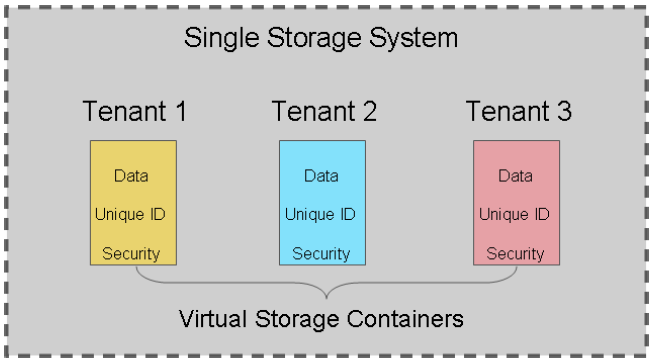
\includegraphics[clip, scale=0.4]{./gfx/virtualstoragecontainer.png}
	\caption[Virtual Storage Container]{Attributes of a Virtual Storage Container \cite{feresten2010}}
	\label{fig:virtualstoragecontainer}
\end{figure}

In this diploma thesis we must take into account the different approaches that most of the Cloud storage vendors have taken into account, in order to provide the tenant transparent access through the \ac{ESB} to his virtual storage container in one or more Cloud infrastructures.